% !TeX encoding = UTF-8

\documentclass{protokol}


\usepackage{tikz}
\usetikzlibrary{calc}
\usetikzlibrary{arrows}

%====== Units =====
\usepackage{siunitx}
\sisetup{inter-unit-product =\ensuremath{\cdot}}
\sisetup{group-digits = integer}
\sisetup{output-decimal-marker = {,}}
\sisetup{exponent-product = \ensuremath{\cdot}}
\sisetup{separate-uncertainty}
\sisetup{tight-spacing = false}
%\sisetup{scientific-notation = true}
%\sisetup{round-mode=places,round-precision=4}
%\sisetup{evaluate-expression}


%====== Grafy =====
\usepackage{pgfplots}
\pgfplotsset{width=0.8\linewidth, compat=1.17}
\def\plotcscale{0.8}
\usepackage{pgfplotstable}
\usepackage[figurename=Obr.]{caption} % figure caption rename

%====== Rovnice align block ======
\usepackage{amsmath}
\setlength{\jot}{10pt} % rozestup mezi řádky

\graphicspath{ {./img/} }

%====== Vyplňte údaje ======
\jmeno{Jakub Charvot}
\kod{240844}
\rocnik{3.}
\obor{MET}
\skupina{MET/2}
\spolupracoval{--}

\merenodne{--}
\odevzdanodne{2.5.\ 2023}
\nazev{Vlastnosti materiálů tlustých vrstev}
\cislo{2} %měřené úlohy

\predmet{Mikroelektronika a technologie součástek}
\ustav{Ústav mikroelektroniky}
\skola{FEKT VUT v~Brně}

\def\para{x+0}
\def\parb{\para-80}


%citace 
\usepackage[backend=biber, style=iso-numeric, sortlocale=cs_CZ, autolang=other, language=czech]{biblatex}
\addbibresource{bibliography.bib}
\DeclareFieldFormat{labelnumberwidth}{\mkbibbrackets{#1}}
% hyperlinky
\usepackage[colorlinks]{hyperref}

% odstavce
\usepackage{parskip}

% Bloky kódu
\usepackage{xcolor}

%New colors defined below
\definecolor{codegreen}{rgb}{0,0.6,0}
\definecolor{codegray}{rgb}{0.5,0.5,0.5}
\definecolor{codepurple}{rgb}{0.58,0,0.82}
\definecolor{backcolour}{rgb}{0.95,0.95,0.92}

\usepackage{listings}
\lstdefinestyle{mystyle}{
  backgroundcolor=\color{backcolour}, commentstyle=\color{codegreen},
  keywordstyle=\color{magenta},
  numberstyle=\tiny\color{codegray},
  stringstyle=\color{codepurple},
  basicstyle=\ttfamily\footnotesize,
  breakatwhitespace=false,         
  breaklines=true,                 
  captionpos=b,                    
  keepspaces=true,                 
  numbers=left,                    
  numbersep=5pt,                  
  showspaces=false,                
  showstringspaces=false,
  showtabs=false,                  
  tabsize=2
}
\lstset{
	inputencoding=utf8,
	extendedchars=true,
	literate={á}{{\'a}}1 {č}{{\v{c}}}1 {ď}{{\v{d}}}1 {é}{{\'e}}1 {ě}{{\v{e}}}1 
           {í}{{\'i}}1 {ň}{{\v{n}}}1 {ó}{{\'o}}1 {ř}{{\v{r}}}1 {š}{{\v{s}}}1 
           {ť}{{\v{t}}}1 {ú}{{\'u}}1 {ů}{{\r{u}}}1 {ý}{{\'y}}1 {ž}{{\v{z}}}1 
           {Á}{{\'A}}1 {Č}{{\v{C}}}1 {Ď}{{\v{D}}}1 {É}{{\'E}}1 {Ě}{{\v{E}}}1 
           {Í}{{\'I}}1 {Ň}{{\v{N}}}1 {Ó}{{\'O}}1 {Ř}{{\v{R}}}1 {Š}{{\v{S}}}1 
           {Ť}{{\v{T}}}1 {Ú}{{\'U}}1 {Ů}{{\r{U}}}1 {Ý}{{\'Y}}1 {Ž}{{\v{Z}}}1,
	style=mystyle
	}

% Číslování
\pagenumbering{arabic}



% =========================================
% =============== DOKUMENT ================
% =========================================
\begin{document}
	%====== Vygenerování tabulky ======
	\maketitle

\section{Teoretický úvod}
  Teorie potřebná k této úloze vychází z předešlých laboratorních úloh, zejména úlohy 2, kdy jsme měřili hodnoty tlustovrstvých rezistorů v závislosti na různých podobách výpalu a také změnu jejich odporu v závislosti na teplotě. Přijde mi zbytečné uvádět znovu základní informace o samotné technologii nebo výpočtu odporu na čtverec, které již v této době semestru musí znát opravdu každý student, proto bude tato sekce o něco kratší.

\subsection{Dostavování TLV rezistorů}
Co se týče nové teorie věnuje se tato úloha také dostavování (nebo také trimmování) již natištěných rezistorů. 
Jak jsme si již vyzkoušeli na předchozích úlohách, přesnost tisku je velkou neznámou a i při optimalizaci všech dostupných parametrů jsou hodnoty stále poměrně nepřesné. Z tohoto důvodu se s nepřesností v návrhu počítá a tisknou se rezistory s o něco nižšími hodnotami než je požadováno. Následně jsou rezistory měřeny a v průběhu měření je jich část odebrána tak, aby se svou hodnotou více přiblížili požadavku. 

Nejčastějšími způsoby je mechanické osbroušení, obvykle proudem částic korundu nebo křemíku, nebo odpaření vrstvy laserem, většinou typ YAG nebo CO\(_{2}\). 

Pro dostavení je možné vyřezat do tlustovrstvého motivu různé obrazce. Obvykle se volí přímý řez od kraje směrem ke středu. Pokud se takovýchto provede více vedle a naproti sobě, vznikne serpentýnový motiv. Alternativou je ještě výřez ve tvaru L \cite{zadani,schroeder2022trimming}.

\section{Praktická část}
\subsection{Test hodnoty vytvořených rezistorů}
  Měřili jsme hodnoty elektrického odporu pro různé vzorky tlustovrstvých rezistorů. V prvním kroku jsme měli k dispozici rezistory o aktivní ploše 3 čtverce ve čtyřech různých variantách -- bez a nebo s použitím krycí vrstvy; vypálené postupně, tedy po vrstvách, a nebo všechny vrstvy současně. V každé variantě jsme měřili 9 vzorků. Ve druhém kroku jsme pak měřili dvě shodné řady rezistorů s rostoucí aktivní plochou, jedna řada byla opatřena krycí vrstvou. 
Přehled měřených variant se nachází v Tab.~\ref{tab:r_varianty}. 
K měření byl použit digitální RLC metr (TODO).

\begin{table}[h!]
    \caption{Přehled jednotlivých měření odporu.}
    \centering
    \def\arraystretch{1.4}
    \begin{tabular}{l|l|l|l|l|l|l}
        Č. varianty  & R1       & R2       & R3       & R4       & R5       & R6       \\ \hline
        Plocha [sq]  & 3        & 3        & 3        & 3        & různá    & různá    \\ \hline
        Krycí vrstva & NE       & ANO      & NE       & ANO      & NE       & ANO      \\ \hline
        Typ výpalu   & najednou & najednou & postupně & postupně & najednou & najednou \\ 
        \end{tabular}
    \label{tab:r_varianty}
\end{table}

Z naměřených hodnot jsme vždy stanovili hodnotu odporu na čtverec. Následně jsme vypočetli průměrnou hodnotu \(\overline{x} \), výběrovou směrodatnou odchylku \(s_{x} \) a variační koeficient \(VK\). Jelikož byla k tisku použita odporová pasta s hodnotou vrstvového odporu \qty{100}{\ohm\per sq} [zdrojem je studentův odhad, protože konkrétní typ použité pasty nám nebyl odhalen], můžeme naměřené hodnoty porovnat také s touto hodnotou, stanovili jsme tedy i relativní odchylku průměrné hodnoty od této teoretické \(\Delta_{r} \).
Naměřené hodnoty a zmíněné statistické údaje pro jednotlivá měření se nacházejí v Tab.~\ref{tab:r1_hodnoty} -- \ref{tab:r6_hodnoty}.


% R1
\begin{table}[h!]
    \caption{Série měření R1 -- Naměřené a zpracované hodnoty.}
    \centering
    \def\arraystretch{1.4}
    \begin{tabular}{l|l|l}
                            & R [\unit{\ohm}]    & \(R_{sq}\) [\unit{\ohm\per sq}]  \\ \hline\hline
                            & 333,82 & 111,27 \\ \hline
                            & 329,55 & 109,85 \\ \hline
                            & 346,68 & 115,56 \\ \hline
                            & 334,16 & 111,39 \\ \hline
                            & 343,70 & 114,57 \\ \hline
                            & 339,74 & 113,25 \\ \hline
                            & 346,30 & 115,43 \\ \hline
                            & 325,41 & 108,47 \\ \hline
                            & 312,67 & 104,22 \\ \hline\hline
        \(x_{teor} \) [\unit{\ohm}]      & 300    & 100    \\ \hline
        \(\overline{x} \) [\unit{\ohm}]  & 334,67 & 111,56 \\ \hline
        \(\Delta_{r} \) [\unit{\percent}]    & 11,56\%& 11,56\%\\ \hline\hline
        \(s_{x} \) [\unit{\ohm}, \unit{\ohm\per sq}]         & 10,45  & 3,48   \\ \hline
        VK [\unit{\percent}]                 & 3,12\% & 3,12\% \\ 
    \end{tabular}
    \label{tab:r1_hodnoty}
\end{table}

%R2
\begin{table}[h!]
    \caption{Série měření R2 -- Naměřené a zpracované hodnoty.}
    \centering
    \def\arraystretch{1.4}
    \begin{tabular}{l|l|l}
                            & R [\unit{\ohm}]    & \(R_{sq}\) [\unit{\ohm\per sq}]  \\ \hline\hline
                            & 1217,6 & 405,87 \\ \hline
                            & 1276,3 & 425,43 \\ \hline
                            & 1321,6 & 440,53 \\ \hline
                            & 1265,7 & 421,90 \\ \hline
                            & 1328,6 & 442,87 \\ \hline
                            & 1389,5 & 463,17 \\ \hline
                            & 1451,6 & 483,87 \\ \hline
                            & 1306,2 & 435,40 \\ \hline
                            & 1061,1 & 353,70 \\ \hline\hline
        \(x_{teor} \) [\unit{\ohm}]      & 300    & 100    \\ \hline
        \(\overline{x} \) [\unit{\ohm}]  & 1290,91  & 430,30 \\ \hline
        \(\Delta_{r} \) [\unit{\percent}]    &  330,30\%& 330,30\%\\ \hline\hline
        \(s_{x} \) [\unit{\ohm}, \unit{\ohm\per sq}]         &  103,91  & 34,64   \\ \hline
        VK [\unit{\percent}]                 &  8,05\% & 8,05\% \\ 
    \end{tabular}
    \label{tab:r2_hodnoty}
\end{table}

% R3
\begin{table}[h!]
    \caption{Série měření R3 -- Naměřené a zpracované hodnoty.}
    \centering
    \def\arraystretch{1.4}
    \begin{tabular}{l|l|l}
                                                      & R [\unit{\ohm}]    & \(R_{sq}\) [\unit{\ohm\per sq}]  \\ \hline\hline
                                                      & 355,03 & 118,34 \\ \hline
                                                      & 348,78 & 116,26 \\ \hline
                                                      & 361,69 & 120,56 \\ \hline
                                                      & 346,98 & 115,66 \\ \hline
                                                      & 346,19 & 115,40 \\ \hline
                                                      & 363,28 & 121,09 \\ \hline
                                                      & 361,12 & 120,37 \\ \hline
                                                      & 349,22 & 116,41 \\ \hline
                                                      & 335,97 & 111,99 \\ \hline\hline
        \(x_{teor} \) [\unit{\ohm}]                   & 300    & 100    \\ \hline
        \(\overline{x} \) [\unit{\ohm}]               & 352,03 & 117,34 \\ \hline
        \(\Delta_{r} \) [\unit{\percent}]             & 17,34\%& 17,34\%\\ \hline\hline
        \(s_{x} \) [\unit{\ohm}, \unit{\ohm\per sq}]  & 8,48   & 2,83   \\ \hline
        VK [\unit{\percent}]                          & 2,41\% & 2,41\% \\ 
    \end{tabular}
    \label{tab:r3_hodnoty}
\end{table}

% R4
\begin{table}[h!]
    \caption{Série měření R4 -- Naměřené a zpracované hodnoty.}
    \centering
    \def\arraystretch{1.4}
    \begin{tabular}{l|l|l}
                                                      & R [\unit{\ohm}]    & \(R_{sq}\) [\unit{\ohm\per sq}]  \\ \hline\hline
                                                      & 363,15 & 121,05 \\ \hline
                                                      & 350,85 & 116,95 \\ \hline
                                                      & 388,36 & 129,45 \\ \hline
                                                      & 364,01 & 121,34 \\ \hline
                                                      & 375,37 & 125,12 \\ \hline
                                                      & 375,08 & 125,03 \\ \hline
                                                      & 368,63 & 122,88 \\ \hline
                                                      & 382,58 & 127,53 \\ \hline
                                                      & 380,45 & 126,82 \\ \hline\hline
        \(x_{teor} \) [\unit{\ohm}]                   & 300    & 100    \\ \hline
        \(\overline{x} \) [\unit{\ohm}]               & 372,05 & 124,02 \\ \hline
        \(\Delta_{r} \) [\unit{\percent}]             & 24,02\%& 24,02\%\\ \hline\hline
        \(s_{x} \) [\unit{\ohm}, \unit{\ohm\per sq}]  & 10,92   & 3,64   \\ \hline
        VK [\unit{\percent}]                          & 2,93\% & 2,93\% \\ 
    \end{tabular}
    \label{tab:r4_hodnoty}
\end{table}

% R5
\begin{table}[h!]
    \caption{Série měření R5 -- Naměřené a zpracované hodnoty.}
    \centering
    \def\arraystretch{1.4}
    \begin{tabular}{l|l|l}
        Akt. plocha [sq]                              & R [\unit{\ohm}]    & \(R_{sq}\) [\unit{\ohm\per sq}]  \\ \hline\hline
        1                                             & 68,56   & 68,56 \\ \hline
        2                                             & 189,09  & 94,55 \\ \hline
        3                                             & 307,82  & 102,61 \\ \hline
        4                                             & 429,70  & 107,43 \\ \hline
        5                                             & 558,80  & 111,76 \\ \hline
        6                                             & 683,00  & 113,83 \\ \hline
        7                                             & 805,40  & 115,06 \\ \hline
        8                                             & 922,00  & 115,25 \\ \hline
        9                                             & 1006,90 & 111,88 \\ \hline\hline
        \(x_{teor} \) [\unit{\ohm}]                   & --      & 100    \\ \hline
        \(\overline{x} \) [\unit{\ohm}]               & --      & 104,55 \\ \hline
        \(\Delta_{r} \) [\unit{\percent}]             & --      & 4,55\%\\ \hline\hline
        \(s_{x} \) [\unit{\ohm}, \unit{\ohm\per sq}]  & --      & 14,24   \\ \hline
        VK [\unit{\percent}]                          & --      & 13,62\% \\ 
    \end{tabular}
    \label{tab:r5_hodnoty}
\end{table}

% R6
\begin{table}[h!]
    \caption{Série měření R6 -- Naměřené a zpracované hodnoty.}
    \centering
    \def\arraystretch{1.4}
    \begin{tabular}{l|l|l}
        Akt. plocha [sq]                              & R [\unit{\ohm}]    & \(R_{sq}\) [\unit{\ohm\per sq}]  \\ \hline\hline
        1                                             & 102,83   & 102,83 \\ \hline
        2                                             & 497,50   & 248,75 \\ \hline
        3                                             & 944,80   & 314,93 \\ \hline
        4                                             & 1428,10  & 357,03 \\ \hline
        5                                             & 1936,60  & 387,32 \\ \hline
        6                                             & 2443,30  & 407,22 \\ \hline
        7                                             & 3089,40  & 441,34 \\ \hline
        8                                             & 3551,40  & 443,93 \\ \hline
        9                                             & 4095,00  & 455,00 \\ \hline\hline
        \(x_{teor} \) [\unit{\ohm}]                   & --       & 100    \\ \hline
        \(\overline{x} \) [\unit{\ohm}]               & --       & 350,93 \\ \hline
        \(\Delta_{r} \) [\unit{\percent}]             & --       & 250,93\%\\ \hline\hline
        \(s_{x} \) [\unit{\ohm}, \unit{\ohm\per sq}]  & --       & 108,26   \\ \hline
        VK [\unit{\percent}]                          & --       & 30,85\% \\ 
    \end{tabular}
    \label{tab:r6_hodnoty}
\end{table}
  \clearpage
\subsection{Test hodnoty kapacity vytvořených kondenzátorů}
  V této části jsme měřili hodnoty kapacit kondenzátorů vytvořených za pomoci tlustovrstvé technologie, konkrétně s použitím dielekrické pasty ESL 4917. Měřeny byly opět LCR metrem (BK Precision 880)
Abychom ověřili přesnost těchto kondenzátorů, je potřeba vypočítat teoretickou hodnotu kapacity, které by měl ideální kondenzátor dosáhnout. Vyjdeme ze známého vztahu:
\[
    C=\varepsilon_{0}\cdot\varepsilon_{r}\cdot\frac{S}{d}
\] 




Katalogový list použité pasty \cite{pastaDatasheet} uvádí pro permitivitu a typickou tloušťku vrstvy vždy rozsah hodnot, viz Tab.~\ref{tab:pasta_hodnoty_katalog}. Pro teoretický výpočet kapacity použijeme tedy vždy okrajové hodnoty:
\[
    C_{teor MAX} = \varepsilon_{0}\cdot\varepsilon_{r MAX}\cdot\frac{S}{d_{MIN} }
\]
\[
    C_{teor MIN} = \varepsilon_{0}\cdot\varepsilon_{r MIN}\cdot\frac{S}{d_{MAX} }
\]

\begin{table}[h!]
    \caption{Výňatek z katalogového listu pasty ESL 4917.}
    \centering
    \def\arraystretch{1.4}
    \begin{tabular}{l|l}
        \(d_{MIN} \)            & \qty{35}{\micro\meter} \\ \hline
        \(d_{MAX} \)            & \qty{50}{\micro\meter} \\ \hline
        \(\varepsilon_{MIN} \)  & 8                      \\ \hline
        \(\varepsilon_{MAX} \)  & 11                     \\ 
        \end{tabular}
    \label{tab:pasta_hodnoty_katalog}
\end{table}

Dále jsme pro každý kondenzátor vypočetli kapacitu na čtverec. Stejný postup byl opakován ve dvou variantách, nejprve pro kondenzátory s vrstvami vypálenými současně (viz Tab. \ref{tab:c_najednou_hodnoty}), poté pro kondenzátory s vrstvami vypalovanými postupně (viz Tab. \ref{tab:c_postupne_hodnoty}). 

Naměřené a vypočtené hodnoty pro obě série měření se nacházejí v Tab.~\ref{tab:c_najednou_hodnoty} a \ref{tab:c_postupne_hodnoty}.

% C najednou
\begin{table}[h!]
    \caption{Teoretické a měřené hodnoty pro kondenzátory s výpalem najednou.}
    \centering
    \def\arraystretch{1.4}
    \begin{tabular}{l|l|l||l|l}
        S [sq] & \(C_{meas} \) [\unit{\pico\farad}] & \(C_{sq} \) [\unit{\pico\farad\per sq}]  & \(C_{teor MIN}\) [\unit{\pico\farad}] & \(C_{teor MAX}\) [\unit{\pico\farad}]\\ \hline
        4      & 11,7   & 2,93  & 5,667     & 11,13    \\ \hline
        25     & 53,4   & 2,14  & 35,42     & 69,57    \\ \hline
        50     & 104,9  & 2,10  & 70,83     & 139,14   \\ \hline
        100    & 203,0  & 2,03  & 141,67    & 278,27   \\ \hline
        200    & 406,7  & 2,03  & 283,33    & 556,55   \\ 
        \end{tabular}
    \label{tab:c_najednou_hodnoty}
\end{table}
\vspace{100pt}
% C postupně
\begin{table}[t!]
    \caption{Teoretické a měřené hodnoty pro kondenzátory s výpalem postupně.}
    \centering
    \def\arraystretch{1.4}
    \begin{tabular}{l|l|l||l|l}
        S [sq] & \(C_{meas} \) [\unit{\pico\farad}] & \(C_{sq} \) [\unit{\pico\farad\per sq}]  & \(C_{teor MIN}\) [\unit{\pico\farad}] & \(C_{teor MAX}\) [\unit{\pico\farad}]\\ \hline
        4       & 14,3  & 3,58  & 5,67       & 11,13   \\ \hline
        25      & 67,5  & 2,70  & 35,42      & 69,57   \\ \hline
        50      & 133,1 & 2,66  & 70,83      & 139,14  \\ \hline
        100     & --    & --    & 141,67     & 278,27  \\ \hline
        200     & 499,3 & 2,50  & 283,33     & 556,55  \\ 

        \end{tabular}
    \label{tab:c_postupne_hodnoty}
\end{table}
  \clearpage
\subsection{Určení velikosti částic v pastě}
  V této části úlohy nám byly předloženy tři vzorky neznámých past a za pomoci grindometru (ELCOMETER 2050/2) jsme prakticky stanovili velikost zrn v jednotlivých pastách. 
Výsledky našeho pozorování se nachází v Tab.~\ref{tab:grindometr}. Jelikož neznáme přesné názvy jednotlivých past, porovnání zjisštěných hodnot s technickými listy není možné.

\begin{table}[h!]
    \caption{Velikost zrn zjištěná za pomoci grindometru.}
    \centering
    \def\arraystretch{1.4}
    \begin{tabular}{l|l|l}
        Č. pasty    & Typ pasty   & Velikost zrn [\unit{\micro\meter}]   \\ \hline
        1    & neznámý   & 10   \\ \hline
        2    & neznámý   &  8   \\ \hline
        4    & neznámý   & 44   \\ 
        \end{tabular}
    \label{tab:grindometr}
\end{table}
  \clearpage
\subsection{Test vazby vrstvy na substrát}
  Za pomoci přístroje Scratch Tester jsme testovali vazbu různých tlustovrstvých past na substrát (Alumina). Přístroj nabízí možnost progresivního testu, při kterém je postupně zvyšována normálová síla (\(F_{Z} \) ). Ve výsledných datech z přístroje jsou k dispozici hodnoty této síly, síly v ose pohybu (\(F_{X} \)) a hodnotu akustické emise smímané mikrofonem, z té by mělo být zjistitelné, jestli došlo k delaminaci vrstvy \cite{DiplomkaScratchTester}. Všechny tyto hodnoty přístroj dává vždy přiřazené ke konkrétní poloze hrotu. 

Testovali jsme tři typy past, získané hodnoty jsou zobrazeny na Obr.~\ref{graf:cermet} (Cermetová pasta), Obr.~\ref{graf:Polymer} (Polymerová pasta) a Obr.~\ref{graf:Rezinat} (Rezinátová pasta).

Následně jsme vytvořenou rýhu analyzovali mikroskopem (Jenavert). Detail pozorovaných deformací je zobrazen na Obr.~\ref{fig:cer1-jpg} (Cermetová pasta), Obr.~\ref{fig:pol1-jpg} (Polymerová pasta) a Obr.~\ref{fig:rez1-jpg} a \ref{fig:rez2-jpg} (Rezinátová pasta).

% Cermet
\begin{figure*}[h!]
    \begin{tikzpicture}
        \centering
        \begin{axis}
            [
            xlabel={ Pozice\ [\unit{\milli\meter}]},
            ylabel={ F \ [\unit{\milli\newton}]},
            axis y line*=left, % dve y osy
            width=1\textwidth,
            height = 0.5\textwidth,
            legend pos=north west
%			xmin=0,
%			ymin=0,
%			xmax=100,
%			ymax=100
            ]
            \addplot[mark=none, mark options={solid}, thick, blue, solid, mark size=3pt] table [skip first n=2, x=A, y=B, col sep=comma] {data/scratchtest/Cermet.csv};
            \addlegendentry{Force Z}

            \addplot[mark=none, mark options={solid}, thick, red, solid, mark size=3pt] table [skip first n=2, x=A, y=D, col sep=comma] {data/scratchtest/Cermet.csv};
            \addlegendentry{Force X}
        \end{axis}   
     
        
%         % Second y axis 
        \begin{axis}
            [
            ylabel={Akustické emise\ [\unit{\decibel}]},
            axis x line=none,
            axis y line*=right,
            width=1\textwidth,
            height = 0.5\textwidth,
            legend pos=north east
%			xmin=0,
%			ymin=0,
%			xmax=100
%			ymax=100
            ]

            \addplot[mark= none, mark options={solid}, thick,  green, dotted, mark size=3pt] table [skip first n=2, x=A, y=C, col sep=comma] {data/scratchtest/Cermet.csv};
            
            \addlegendentry{Akustické emise}
        \end{axis}   
    \end{tikzpicture}
    \caption{Scratch test -- Cermet.}
    \label{graf:cermet}
\end{figure*}

% Polymer
\begin{figure*}[h!]
    \begin{tikzpicture}
        \centering
        \begin{axis}
            [
            xlabel={ Pozice\ [\unit{\milli\meter}]},
            ylabel={ F \ [\unit{\milli\newton}]},
            axis y line*=left, % dve y osy
            width=1\textwidth,
            height = 0.5\textwidth,
            legend pos=north west
%			xmin=0,
%			ymin=0,
%			xmax=100,
%			ymax=100
            ]
            \addplot[mark=none, mark options={solid}, thick, blue, solid, mark size=3pt] table [skip first n=2, x=A, y=B, col sep=comma] {data/scratchtest/Polymer.csv};
            \addlegendentry{Force Z}

            \addplot[mark=none, mark options={solid}, thick, red, solid, mark size=3pt] table [skip first n=2, x=A, y=D, col sep=comma] {data/scratchtest/Polymer.csv};
            \addlegendentry{Force X}
        \end{axis}   
     
        
%         % Second y axis 
        \begin{axis}
            [
            ylabel={Akustické emise\ [\unit{\decibel}]},
            axis x line=none,
            axis y line*=right,
            width=1\textwidth,
            height = 0.5\textwidth,
            legend pos=north east
%			xmin=0,
%			ymin=0,
%			xmax=100
%			ymax=100
            ]

            \addplot[mark= none, mark options={solid}, thick,  green, dotted, mark size=3pt] table [skip first n=2, x=A, y=C, col sep=comma] {data/scratchtest/Polymer.csv};
            
            \addlegendentry{Akustické emise}
        \end{axis}   
    \end{tikzpicture}
    \caption{Scratch test -- Polymer.}
    \label{graf:Polymer}
\end{figure*}

% Rezinat
\begin{figure*}[h!]
    \begin{tikzpicture}
        \centering
        \begin{axis}
            [
            xlabel={ Pozice\ [\unit{\milli\meter}]},
            ylabel={ F \ [\unit{\milli\newton}]},
            axis y line*=left, % dve y osy
            width=1\textwidth,
            height = 0.5\textwidth,
            legend pos=north west
%			xmin=0,
%			ymin=0,
%			xmax=100,
%			ymax=100
            ]
            \addplot[mark=none, mark options={solid}, thick, blue, solid, mark size=3pt] table [skip first n=2, x=A, y=B, col sep=comma] {data/scratchtest/Rezinat.csv};
            \addlegendentry{Force Z}

            \addplot[mark=none, mark options={solid}, thick, red, solid, mark size=3pt] table [skip first n=2, x=A, y=D, col sep=comma] {data/scratchtest/Rezinat.csv};
            \addlegendentry{Force X}
        \end{axis}   
     
        
%         % Second y axis 
        \begin{axis}
            [
            ylabel={Akustické emise\ [\unit{\decibel}]},
            axis x line=none,
            axis y line*=right,
            width=1\textwidth,
            height = 0.5\textwidth,
            legend pos=north east
%			xmin=0,
%			ymin=0,
%			xmax=100
%			ymax=100
            ]

            \addplot[mark= none, mark options={solid}, thick,  green, dotted, mark size=3pt] table [skip first n=2, x=A, y=C, col sep=comma] {data/scratchtest/Rezinat.csv};
            
            \addlegendentry{Akustické emise}
        \end{axis}   
    \end{tikzpicture}
    \caption{Scratch test -- Rezinát.}
    \label{graf:Rezinat}
\end{figure*}


\begin{figure}[h!]
    \centering
    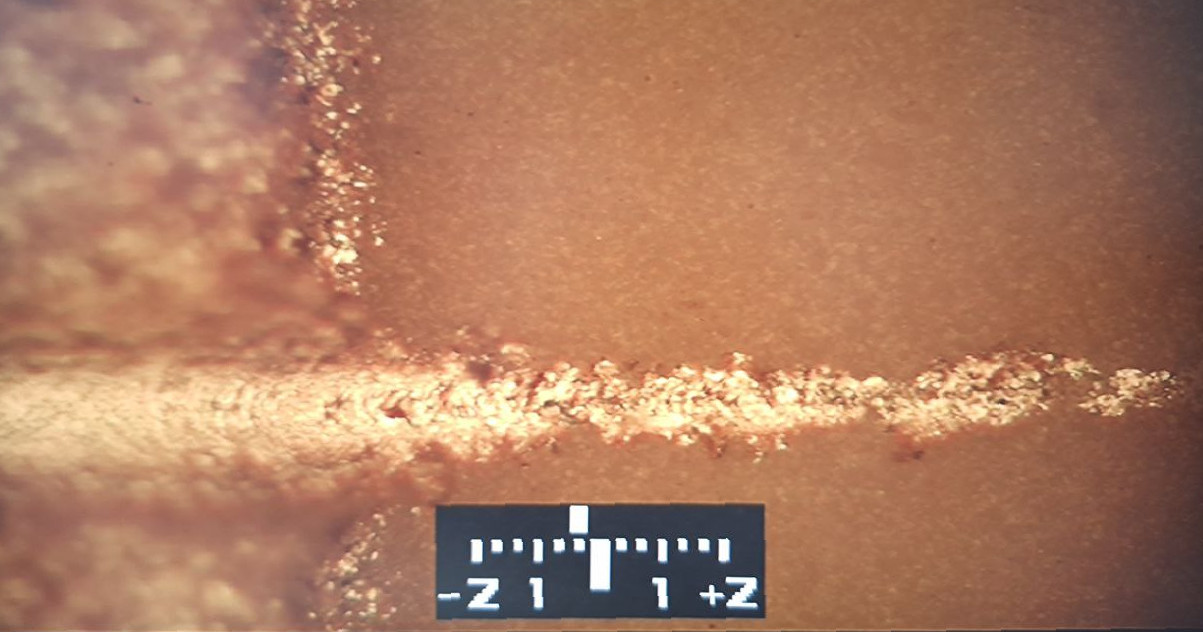
\includegraphics[width=0.8\textwidth]{cer1.jpg}
    \caption{Cermetová pasta po scratch testu (Jenavert).}
    \label{fig:cer1-jpg}
\end{figure}


\begin{figure}[h!]
    \centering
    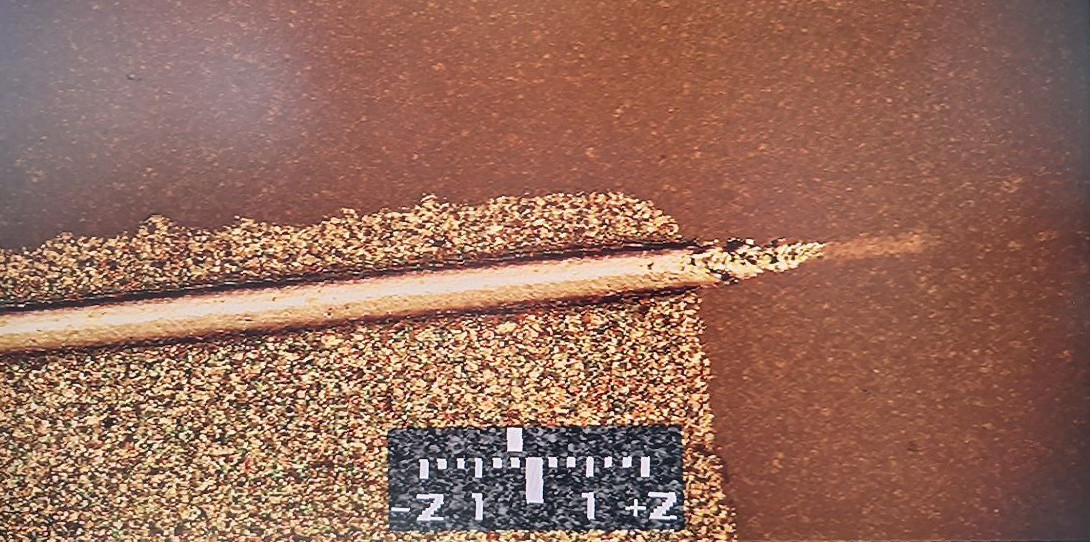
\includegraphics[width=0.8\textwidth]{pol1.jpg}
    \caption{Polymerová pasta po scratch testu (Jenavert).}
    \label{fig:pol1-jpg}
\end{figure}

\begin{figure}[h!]
    \centering
    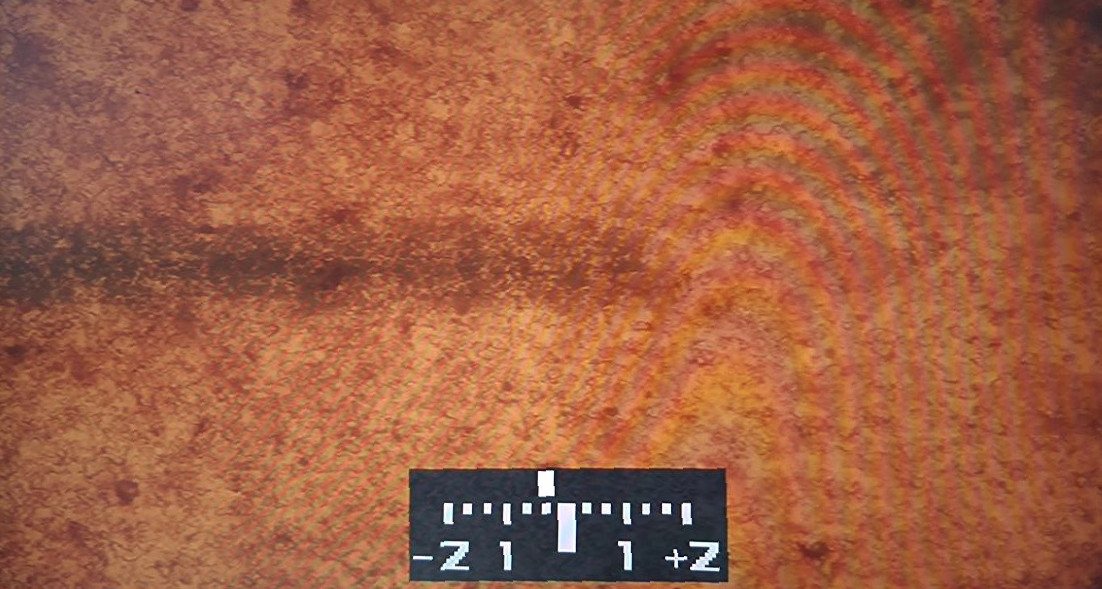
\includegraphics[width=0.8\textwidth]{rez1.jpg}
    \caption{Rezinátová pasta po scratch testu (Jenavert).}
    \label{fig:rez1-jpg}
\end{figure}

\begin{figure}[h!]
    \centering
    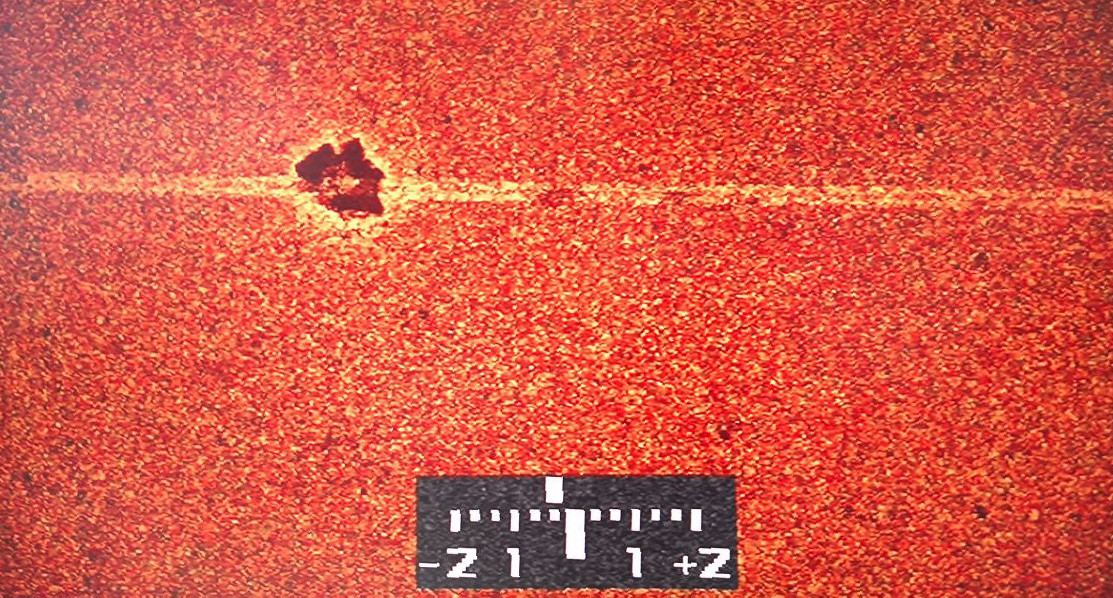
\includegraphics[width=0.8\textwidth]{rez4.jpg}
    \caption{Rezinátová pasta -- delaminace (Jenavert).}
    \label{fig:rez2-jpg}
\end{figure}
  \clearpage

\section{Závěr}
  Jak je vidět z grafů a tubulky naměřených hodnot, pro některé série jsou výsledky v různých kvadrantech obdobné, pro některé naopak vůbec. Nejhomogennějšíh výsledku dosáhla série RX\_3. Také je vidět, že napříč sériemi vycházely celkově o něco menší hodnoty v prvním kvadrantu a naopak vyšší ve druhém a třetím. 

Při porovnání naměřených hodnot s teoretickými se ale dostáváme do prekérní situace. Odchylka zde dosahuje několika řádů kdy namísto stovek \unit{\ohm} měříme hodnoty i v nižších stovkách \unit{\mega\ohm}, typycky pak v jednotkách \unit{\mega\ohm}. Toto nasvědčuje buďto hrubé systematické chybě měření neno špatným informacím ohledně použité odporové pasty, popř. kombinaci obou faktorů. Vzhledem k tomu, že měření bylo prováděno poměrně dlouhý čas a dohlíženo čtyřmi osobami se mi takto hruhá chyba jeví jako nepravděpodobná, ovšem vyloučna není. 
  

\section*{Reference}
\printbibliography[heading=none]

% \clearpage

% \section*{Přílohy}

% \appendix % příkaz pro začátek sekce příloh
% \section{SPICE model \textbf{AD633} (ad633.lib)}
% \label{priloha:spicemodel}
% \lstinputlisting{../ad633.lib}

% \section{Ngspice kód pro simulace v~tomto projektu (projekt.cir)}
% \label{priloha:projekt.cir}
% \lstinputlisting{../projekt.cir}

% \(\) 
% \section{Výsledky fourierovy analýzy ve vlastním experimentu (\ref{sekce:vlastni-experiment})}
% \label{priloha:fourier-data}
% \subsection{\(f_{signal} =\)\qty{10}{\hertz}}
% \lstinputlisting{data/f/fourier_output10k+.txt}

% \subsection{\(f_{signal} =\)\qty{100}{\hertz}}
% \lstinputlisting{data/f/fourier_output100+.txt}

% \subsection{\(f_{signal} =\)\qty{1}{\kilo\hertz}}
% \lstinputlisting{data/f/fourier_output1k+.txt}

% \subsection{\(f_{signal} =\)\qty{10}{\kilo\hertz}}
% \lstinputlisting{data/f/fourier_output10+.txt}

% \subsection{\(f_{signal} =\)\qty{100}{\kilo\hertz}}
% \lstinputlisting{data/f/fourier_output100k+.txt}

\end{document}